% A simple template for LaTeX documents
% 
% To produce pdf run:
%   $ pdflatex paper.tex 
%

\documentclass[12pt]{article}

% Begin paragraphs with new line
\usepackage{parskip}  

% Change margin size
\usepackage[margin=1in]{geometry}   

% Graphics Example:  (PDF's make for good plots)
\usepackage{graphicx}               
% \centerline{\includegraphics{figure.pdf}}

% Allows hyperlinks
\usepackage{hyperref}

% Blocks of code
\usepackage{listings}
\lstset{basicstyle=\ttfamily, title=\lstname}
% Insert code like this. replace `plot.R` with file name.
% \lstinputlisting{plot.R}

% Supports proof environment
\usepackage{amsthm}

% Allows writing \implies and align*
\usepackage{amsmath}

% Allows mathbb{R}
\usepackage{amsfonts}


%%%%%%%%%%%%%%%%%%%%%%%%%%%%%%%%%%%%%%%%%%%%%%%%%%%%%%%%%%%%
\begin{document}

\title{US Korea Exchange Rates \\ STA206 Final Project}
\date{December 15, 2014}
\author{Clark Fitzgerald clarkfitzg@gmail.com \\ 
        Amy Kim atykim@ucdavis.edu}

\maketitle

\begin{abstract}
    We analyze the exchange rate between the United States and South Korea
    (hereafter Korea) using monthly country level economic data.
\end{abstract}

\section{Introduction}

\subsection{Background}

In today's highly connected global society people and money move between
countries. The exchange rates between countries determine the relative
value of that money.

We analyze data on exchange rate between the US and Korea from 1999 to
2014. In 1997 the IMF crisis in Korea perturbed the economic indicators,
but in looking at the data we can see that it has been stable since 1999.

\subsection{Questions}

\begin{enumerate}

    \item How do exchange rates behave?

    \item Can we predict the exchange rate between two countries?  

    \item When is the best time to exchange currency from won (Korean
        currency) to dollar or vice versa?  

    \item Can we find a linear relationship
        that can be applied over other countries' currency? 

\end{enumerate}

\subsection{Motivation}

Sometimes it's necessary to transfer funds between countries. This is true
for both individuals, families, and organizations. The exchange rate can
vary substantially over time. For example, in
Figure~\ref{fig:exchange_rate} we observe the exchange rate between Korea
and the US varying between 900 and 1400 Korean Won per US Dollar. A quick
calculation on this data 
implies that during this period a fixed amount of Korean currency 
could have been worth \$100,000 or \$158,000, depending on when it was  
exchanged. 

Hence if one has a significant amount of capital to move from
one country to another and some flexibility around the timing then it makes
sense to do it when the exchange rates
are favorable for the transfer. For example, you may want to sell a
house in Korea and put that money towards a house in the US.

\subsection{Data}

We use data from Quandl.com, a service that provides clean, documented
data from a wide variety of sources including the US Federal Reserve,
World Bank, and the National Bank of Korea. 
{\tt Exchange rate} between Korean Won and US dollar is the primary $Y$
variable.

For each country we will examine the following variables:

\begin{itemize}
    \item {\tt gdp} The gross domestic product. Units: USD Million
    \item {\tt unemployment rate} The percentage of the labor force who are unemployed and actively seeking work. Units: Percent (monthly)
    \item {\tt exports} The total value of the goods and services
produced domestically and purchased by foreign entities. Units: USD Million (Monthly)
    \item {\tt imports} The total value of a country's imports of physical goods and payments to foreigners for services like shipping and tourism. Units: USD Million (Monthly)
    \item {\tt interest rate} The monthly average of the central bank policy rate. This is the interest rate the central bank charges on loans to commercial banks. Units: Percent (Monthly)
    \item {\tt inflation rate} The growth rate of the prices. (Monthly)
    \item {\tt consumer produce index} The Consumer Price Index (CPI) is a measure of inflation related to the cost of living. Units: Index Points 2010=100, NSA (Monthly)
    \item {\tt debt} The total amount of public and private debt owned by foreign creditors. Units: USD Million Current Prices, NSA (quarterly)
    \item {\tt gdp deflator} The relative difference between the real and nominal GDPs. Units: Index Points NSA
    \item {\tt goverment spending} The yearly expenditure of the federal
        government. Units: local currency
    \item {\tt political party} Categorical variable for the political
party of the president.
\end{itemize}

\section{Methods and Results}

\subsection{Dynamic Data}

The data used in this analysis is unusual- it's generated dynamically from
live, high quality sources, and is self updating. The data is loaded directly from Quandl using a REST (Representational 
State Transfer) web API (Application programming interface), and then
cached locally, limiting network dependence.
Using this service makes it easy to repeat the analysis in the future, or conduct similar analyses between
different countries.

\subsection{Reproducibility}

Above we mentioned that the data and all analysis in the report is self 
updating. This is accomplished through the use of GNU \texttt{make}, which
describes a DAG (Directed Acyclic Graph) of dependencies for the final
report. \texttt{make} detects file modifications and will lazily run all
commands and scripts required for the final output.

What does this mean? Suppose that we need more variables to do the
regression. Thanks to the use
of industry standard ISO codes for the countries and proper parameters in
our code base this becomes a simple task.
We've stored string templates for the country level 
variables in a file
called \texttt{template.txt}. The data collection and preprocessing steps
are automated, so we can add more variables simply by adding a row to
\texttt{template.txt} and entering the command \texttt{make} from the shell
prompt, which causes the following sequence of events: 

\begin{enumerate}
    \item \texttt{make} detects the changed template file
    \item The script \texttt{download.R} runs, updating the cache
    \item The script \texttt{preprocess.R} runs, applying the appropriate
        transformations and joining the tables to a form suitable for
        analysis
    \item All other scripts which depend on the preprocessed data run
    \item The report output is produced
\end{enumerate}

In this case the output is a PDF, but it could just as easily be a web page
on the department server, or an upload into another REST API.

If we were doing this analysis for a client and need to run it again a year
later with a new year of data 
then all we have to do is type \texttt{make}. We'll still need to interpret
plots and models, but the most time consuming work is done.

One other aspect of reproducibility is version control. In this
project we've used \texttt{Git} to collect snapshots of the project at
every stage. The project is hosted publicly on
Github\footnote{\url{https://github.com/clarkfitzg/stats206\_project}}.
A look at the log file shows what work happened when and why,
which is important for establishing provenance. In particular it shows 
that we've been active on this project every day since
December 1st. Here's an example of a log entry:

\begin{verbatim}
commit e2beaf01b0a1457e7167989c1fae575c2a676f19
Author: Clark Fitzgerald <clarkfitzg@gmail.com>
Date:   Mon Dec 8 20:51:04 2014 -0800

    implemented local caching, decoupled download step
\end{verbatim}

Through a little engineering the data analysis process
can be made transparent, automated, extensible, and fully reproducible.

Modern high level programming languages like R provide incredible tools. By
using their capabilities we can 

Figure~\ref{fig:correlation} shows a histogram of all the pairwise sample
correlations.

Figure~\ref{fig:na_plot_KOR} shows the variables which were interpolated.

Attempting to reference \cite{lamport94}.

\section{Conclusions and Discussion}


\newpage
\section{Appendix}

\listoffigures

\begin{figure}
  \centering
    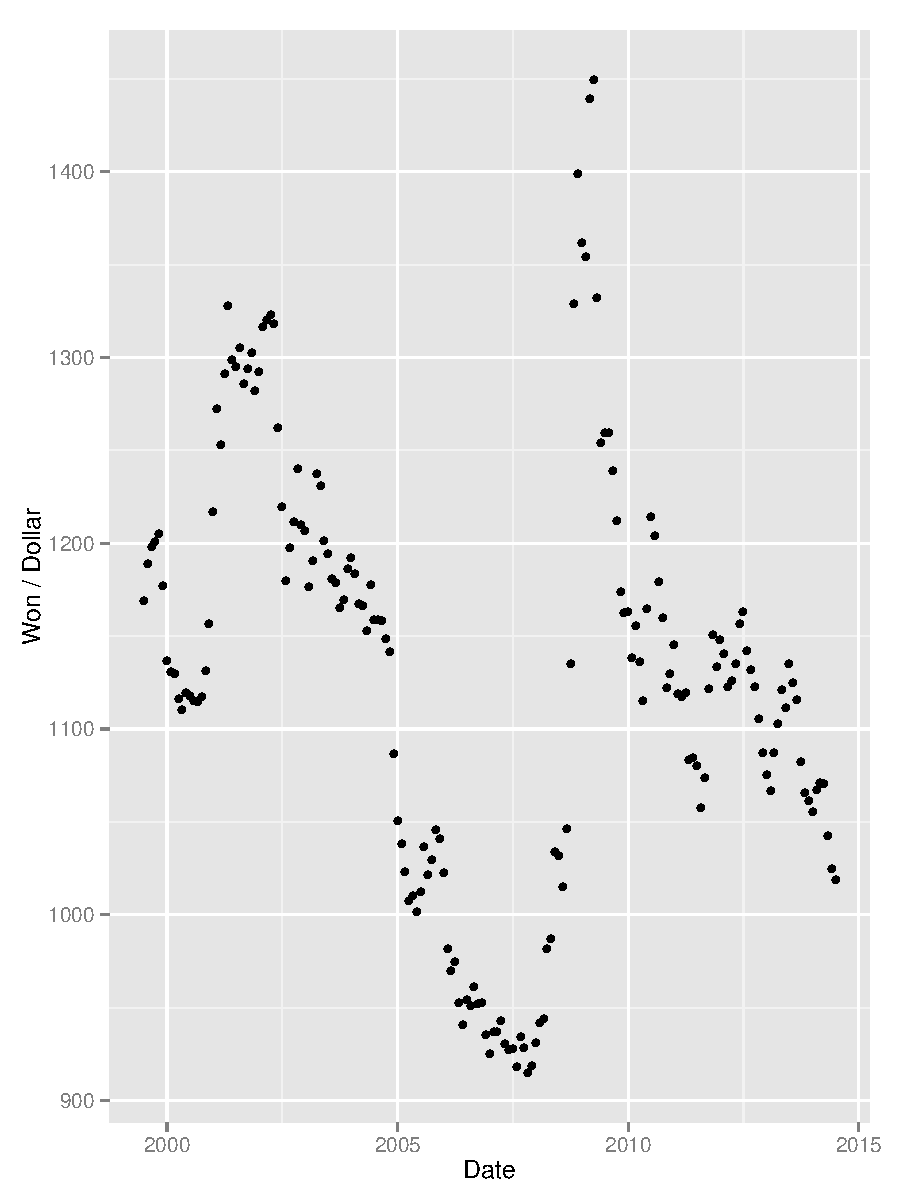
\includegraphics{exchange_rate.pdf}
  \caption{Exchange rate between US and South Korea from 1999 to 2014}
  \label{fig:exchange_rate}
\end{figure}

\begin{figure}
  \centering
    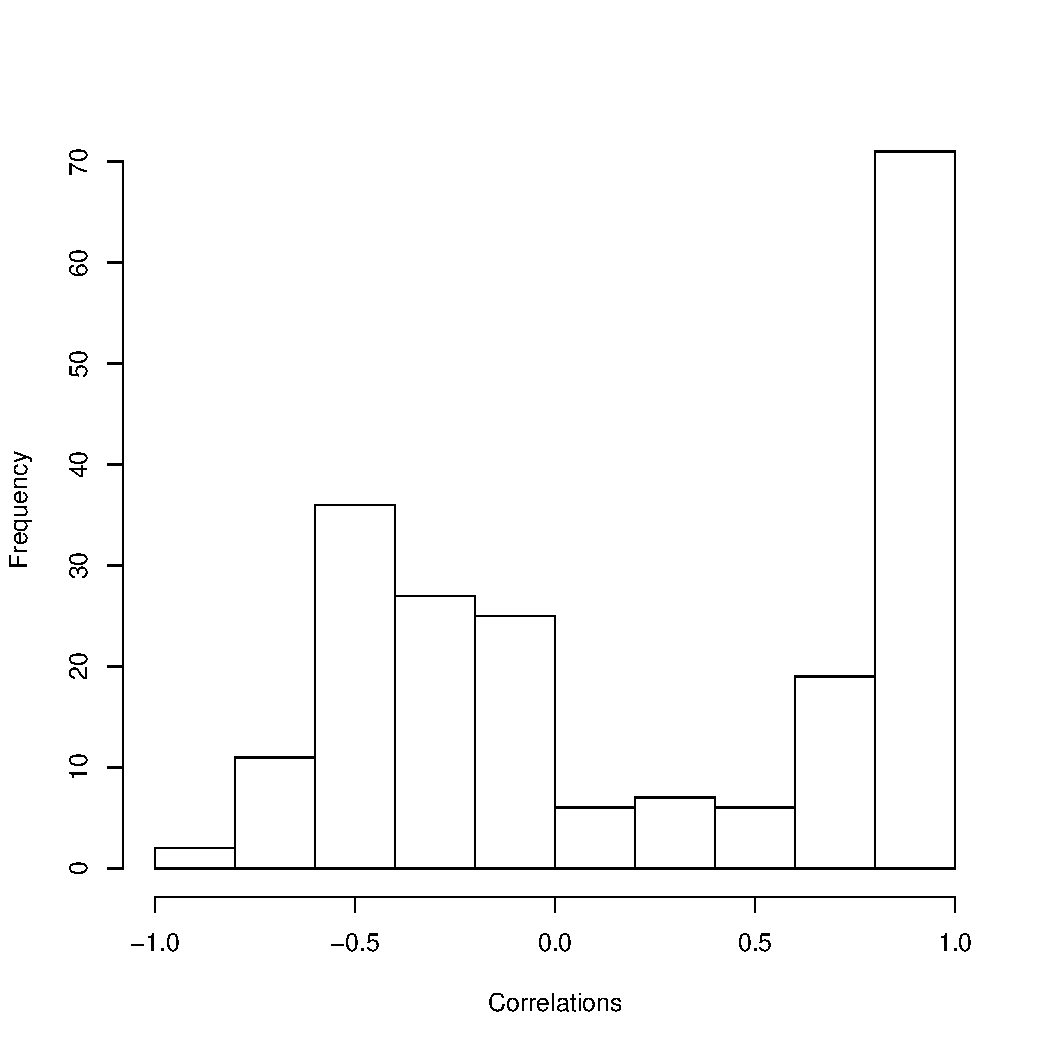
\includegraphics{correlation.pdf}
  \caption{Histogram of all pairwise sample correlations}
  \label{fig:correlation}
\end{figure}

\begin{figure}
  \centering
    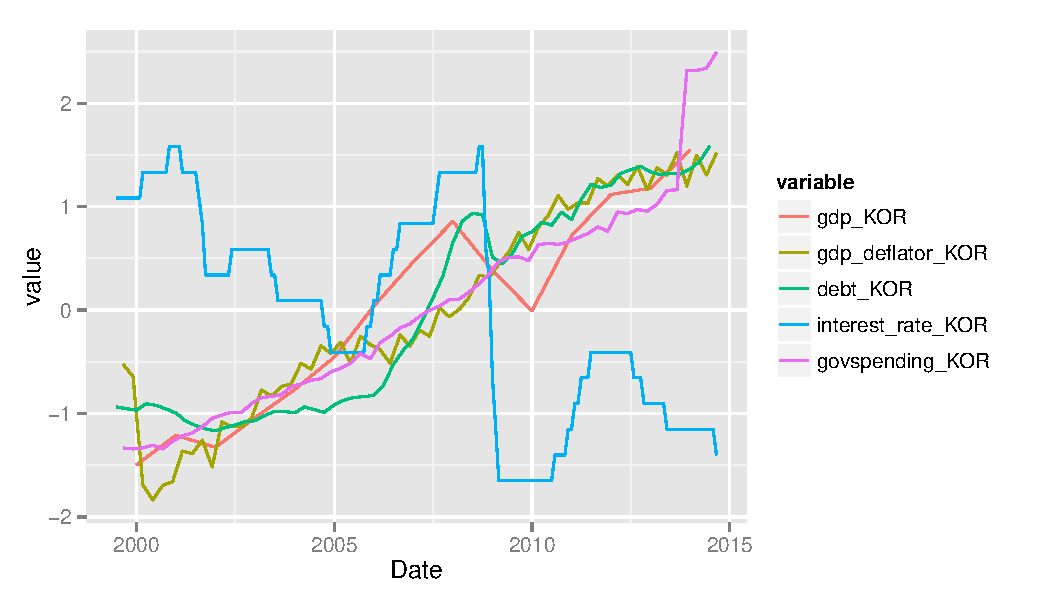
\includegraphics{na_plot_KOR.pdf}
  \caption{Scaled variables with NA values}
  \label{fig:na_plot_KOR}
\end{figure}

\newpage

\begin{thebibliography}{9}

\bibitem{lamport94}
  Leslie Lamport,
  \emph{\LaTeX: a document preparation system}.
  Addison Wesley, Massachusetts,
  2nd edition,
  1994.

\end{thebibliography}

\end{document}
